\documentclass[floatsintext,doc]{apa6}

\usepackage{amssymb,amsmath}
\usepackage{ifxetex,ifluatex}
\usepackage{fixltx2e} % provides \textsubscript
\ifnum 0\ifxetex 1\fi\ifluatex 1\fi=0 % if pdftex
  \usepackage[T1]{fontenc}
  \usepackage[utf8]{inputenc}
\else % if luatex or xelatex
  \ifxetex
    \usepackage{mathspec}
    \usepackage{xltxtra,xunicode}
  \else
    \usepackage{fontspec}
  \fi
  \defaultfontfeatures{Mapping=tex-text,Scale=MatchLowercase}
  \newcommand{\euro}{€}
\fi
% use upquote if available, for straight quotes in verbatim environments
\IfFileExists{upquote.sty}{\usepackage{upquote}}{}
% use microtype if available
\IfFileExists{microtype.sty}{\usepackage{microtype}}{}
\usepackage{color}
\usepackage{fancyvrb}
\newcommand{\VerbBar}{|}
\newcommand{\VERB}{\Verb[commandchars=\\\{\}]}
\DefineVerbatimEnvironment{Highlighting}{Verbatim}{commandchars=\\\{\}}
% Add ',fontsize=\small' for more characters per line
\usepackage{framed}
\definecolor{shadecolor}{RGB}{248,248,248}
\newenvironment{Shaded}{\begin{snugshade}}{\end{snugshade}}
\newcommand{\AlertTok}[1]{\textcolor[rgb]{0.94,0.16,0.16}{#1}}
\newcommand{\AnnotationTok}[1]{\textcolor[rgb]{0.56,0.35,0.01}{\textbf{\textit{#1}}}}
\newcommand{\AttributeTok}[1]{\textcolor[rgb]{0.77,0.63,0.00}{#1}}
\newcommand{\BaseNTok}[1]{\textcolor[rgb]{0.00,0.00,0.81}{#1}}
\newcommand{\BuiltInTok}[1]{#1}
\newcommand{\CharTok}[1]{\textcolor[rgb]{0.31,0.60,0.02}{#1}}
\newcommand{\CommentTok}[1]{\textcolor[rgb]{0.56,0.35,0.01}{\textit{#1}}}
\newcommand{\CommentVarTok}[1]{\textcolor[rgb]{0.56,0.35,0.01}{\textbf{\textit{#1}}}}
\newcommand{\ConstantTok}[1]{\textcolor[rgb]{0.00,0.00,0.00}{#1}}
\newcommand{\ControlFlowTok}[1]{\textcolor[rgb]{0.13,0.29,0.53}{\textbf{#1}}}
\newcommand{\DataTypeTok}[1]{\textcolor[rgb]{0.13,0.29,0.53}{#1}}
\newcommand{\DecValTok}[1]{\textcolor[rgb]{0.00,0.00,0.81}{#1}}
\newcommand{\DocumentationTok}[1]{\textcolor[rgb]{0.56,0.35,0.01}{\textbf{\textit{#1}}}}
\newcommand{\ErrorTok}[1]{\textcolor[rgb]{0.64,0.00,0.00}{\textbf{#1}}}
\newcommand{\ExtensionTok}[1]{#1}
\newcommand{\FloatTok}[1]{\textcolor[rgb]{0.00,0.00,0.81}{#1}}
\newcommand{\FunctionTok}[1]{\textcolor[rgb]{0.00,0.00,0.00}{#1}}
\newcommand{\ImportTok}[1]{#1}
\newcommand{\InformationTok}[1]{\textcolor[rgb]{0.56,0.35,0.01}{\textbf{\textit{#1}}}}
\newcommand{\KeywordTok}[1]{\textcolor[rgb]{0.13,0.29,0.53}{\textbf{#1}}}
\newcommand{\NormalTok}[1]{#1}
\newcommand{\OperatorTok}[1]{\textcolor[rgb]{0.81,0.36,0.00}{\textbf{#1}}}
\newcommand{\OtherTok}[1]{\textcolor[rgb]{0.56,0.35,0.01}{#1}}
\newcommand{\PreprocessorTok}[1]{\textcolor[rgb]{0.56,0.35,0.01}{\textit{#1}}}
\newcommand{\RegionMarkerTok}[1]{#1}
\newcommand{\SpecialCharTok}[1]{\textcolor[rgb]{0.00,0.00,0.00}{#1}}
\newcommand{\SpecialStringTok}[1]{\textcolor[rgb]{0.31,0.60,0.02}{#1}}
\newcommand{\StringTok}[1]{\textcolor[rgb]{0.31,0.60,0.02}{#1}}
\newcommand{\VariableTok}[1]{\textcolor[rgb]{0.00,0.00,0.00}{#1}}
\newcommand{\VerbatimStringTok}[1]{\textcolor[rgb]{0.31,0.60,0.02}{#1}}
\newcommand{\WarningTok}[1]{\textcolor[rgb]{0.56,0.35,0.01}{\textbf{\textit{#1}}}}

% Table formatting
\usepackage{longtable, booktabs}
\usepackage{lscape}
% \usepackage[counterclockwise]{rotating}   % Landscape page setup for large tables
\usepackage{multirow}		% Table styling
\usepackage{tabularx}		% Control Column width
\usepackage[flushleft]{threeparttable}	% Allows for three part tables with a specified notes section
\usepackage{threeparttablex}            % Lets threeparttable work with longtable

% Create new environments so endfloat can handle them
% \newenvironment{ltable}
%   {\begin{landscape}\begin{center}\begin{threeparttable}}
%   {\end{threeparttable}\end{center}\end{landscape}}

\newenvironment{lltable}
  {\begin{landscape}\begin{center}\begin{ThreePartTable}}
  {\end{ThreePartTable}\end{center}\end{landscape}}




% The following enables adjusting longtable caption width to table width
% Solution found at http://golatex.de/longtable-mit-caption-so-breit-wie-die-tabelle-t15767.html
\makeatletter
\newcommand\LastLTentrywidth{1em}
\newlength\longtablewidth
\setlength{\longtablewidth}{1in}
\newcommand\getlongtablewidth{%
 \begingroup
  \ifcsname LT@\roman{LT@tables}\endcsname
  \global\longtablewidth=0pt
  \renewcommand\LT@entry[2]{\global\advance\longtablewidth by ##2\relax\gdef\LastLTentrywidth{##2}}%
  \@nameuse{LT@\roman{LT@tables}}%
  \fi
\endgroup}


  \usepackage{graphicx}
  \makeatletter
  \def\maxwidth{\ifdim\Gin@nat@width>\linewidth\linewidth\else\Gin@nat@width\fi}
  \def\maxheight{\ifdim\Gin@nat@height>\textheight\textheight\else\Gin@nat@height\fi}
  \makeatother
  % Scale images if necessary, so that they will not overflow the page
  % margins by default, and it is still possible to overwrite the defaults
  % using explicit options in \includegraphics[width, height, ...]{}
  \setkeys{Gin}{width=\maxwidth,height=\maxheight,keepaspectratio}
\ifxetex
  \usepackage[setpagesize=false, % page size defined by xetex
              unicode=false, % unicode breaks when used with xetex
              xetex]{hyperref}
\else
  \usepackage[unicode=true]{hyperref}
\fi
\hypersetup{breaklinks=true,
            pdfauthor={},
            pdftitle={Supplement to Action Effects on Visual Perception of Distances: A Multilevel Bayesian Meta-Analysis},
            colorlinks=true,
            citecolor=blue,
            urlcolor=blue,
            linkcolor=black,
            pdfborder={0 0 0}}
\urlstyle{same}  % don't use monospace font for urls

\setlength{\parindent}{0pt}
%\setlength{\parskip}{0pt plus 0pt minus 0pt}

\setlength{\emergencystretch}{3em}  % prevent overfull lines


% Manuscript styling
\captionsetup{font=singlespacing,justification=justified}
\usepackage{csquotes}
\usepackage{upgreek}



\usepackage{tikz} % Variable definition to generate author note

% fix for \tightlist problem in pandoc 1.14
\providecommand{\tightlist}{%
  \setlength{\itemsep}{0pt}\setlength{\parskip}{0pt}}

% Essential manuscript parts
  \title{Supplement to Action Effects on Visual Perception of Distances: A Multilevel Bayesian Meta-Analysis}

  \shorttitle{Supplementary Materials}


  \author{Lisa Molto\textsuperscript{1}, Ladislas Nalborczyk\textsuperscript{1,2}, Richard Palluel-Germain\textsuperscript{1}, \& Nicolas Morgado\textsuperscript{3}}

  % \def\affdep{{"", "", "", ""}}%
  % \def\affcity{{"", "", "", ""}}%

  \affiliation{
    \vspace{0.5cm}
          \textsuperscript{1} Univ. Grenoble Alpes, CNRS, LPNC, 38000 Grenoble, France\\
          \textsuperscript{2} Department of Experimental Clinical and Health Psychology, Ghent University\\
          \textsuperscript{3} Univ. Paris Nanterre, Centre de Recherche sur le Sport et le Mouvement, Nanterre, France  }

  \authornote{
    Correspondence concerning this article should be addressed to Nicolas Morgado, Centre de Recherche sur le Sport et le Mouvement (CeRSM). UFR Sciences et Techniques des Activités Physiques et Sportives (STAPS). 200 av. de la République - 92001 Nanterre Cedex. E-mail: \href{mailto:nicolasmorgado-univparisnanterre@outlook.fr}{\nolinkurl{nicolasmorgado-univparisnanterre@outlook.fr}}
  }


  



  \usepackage{graphicx,pdflscape}
  \usepackage{geometry}
  \usepackage{float}

\begin{document}

\maketitle

\setcounter{secnumdepth}{5}


  {
  \hypersetup{linkcolor=black}
  \setcounter{tocdepth}{3}
  \tableofcontents
  }

\newpage

\hypertarget{the-meta-analytic-model}{%
\section{The meta-analytic model}\label{the-meta-analytic-model}}

Let \(y_{ij}\) be the effect size of the \(i\)th study in the \(j\)th article. Then, the 3-levels meta-analytic model can be written as:

\[
\begin{aligned}
y_{ij} &\sim \mathrm{Normal}(\mu_{ij}, \sigma_{ij}) \\
\mu_{ij} &= \alpha + \alpha_{article[j]} + \alpha_{study[ij]} \\
\alpha_{study[ij]} &\sim \mathrm{Normal}(0, \tau_{s}) \\
\alpha_{article[j]} &\sim \mathrm{Normal}(0, \tau_{a}) \\
\end{aligned}
\]

Where \(\sigma_{ij}^{2}\) is the known sampling variance of the \(i\)th study in the \(j\)th article and \(\alpha\) is the population effect size. The index \(\alpha_{study[ij]}\) indicates the intercept corresponding to study \(i\) in article \(j\) (which is the average effect size in this study), and \(\alpha_{article[j]}\) indicates the intercept for article \(j\) (which is the average effect size in this article). In addition to the sampling variance, there are two other sources of variation: the variance of the effect between studies \(\text{Var}(\alpha_{study}) = \tau_{s}^{2}\) (level-2), and the variance of the effect between articles \(\text{Var}(\alpha_{article}) = \tau_{a}^{2}\) (level-3).

\hypertarget{fitting-the-model}{%
\subsection{Fitting the model}\label{fitting-the-model}}

We can then write the full Bayesian model, including the priors for \(\alpha\) (the intercept) and the variance components. The intercept of the model estimates the overall effect and is given an midly informative normal prior. The variance components \(\tau_{s}\) and \(\tau_{a}\) have midly informative Half-Cauchy priors, ensuring that very large values (which are implausible for the scale of \(y_{ij}\)), receive less prior weight.

\[
\begin{aligned}
y_{ij} &\sim \mathrm{Normal}(\mu_{ij}, \sigma_{ij}) \\
\mu_{ij} &= \alpha + \alpha_{article[j]} + \alpha_{study[ij]} \\
\alpha_{study[ij]} &\sim \mathrm{Normal}(0, \tau_{s}) \\
\alpha_{article[j]} &\sim \mathrm{Normal}(0, \tau_{a}) \\
\alpha &\sim \mathrm{Normal}(0, 1) \\
\tau_{s}, \tau_{a} &\sim \mathrm{HalfCauchy}(0, 0.1) \\
\end{aligned}
\]

This model can easily be fitted using the \texttt{brms} package (Bürkner, 2017), with an lme4-like syntax.

\begin{Shaded}
\begin{Highlighting}[]
\KeywordTok{library}\NormalTok{(tidyverse)}
\KeywordTok{library}\NormalTok{(brms)}

\CommentTok{# setting the seed for reproducibility}
\KeywordTok{set.seed}\NormalTok{(}\DecValTok{123}\NormalTok{)}

\CommentTok{# defining the priors}
\NormalTok{prior1 <-}\StringTok{ }\KeywordTok{c}\NormalTok{(}
    \KeywordTok{prior}\NormalTok{(}\KeywordTok{normal}\NormalTok{(}\DecValTok{0}\NormalTok{, }\DecValTok{1}\NormalTok{), }\DataTypeTok{coef =}\NormalTok{ intercept),}
    \KeywordTok{prior}\NormalTok{(}\KeywordTok{cauchy}\NormalTok{(}\DecValTok{0}\NormalTok{, }\FloatTok{0.1}\NormalTok{), }\DataTypeTok{class =}\NormalTok{ sd)}
\NormalTok{    )}

\NormalTok{bmod1 <-}\StringTok{ }\KeywordTok{brm}\NormalTok{(}
\NormalTok{    g }\OperatorTok{|}\StringTok{ }\KeywordTok{se}\NormalTok{(}\KeywordTok{sqrt}\NormalTok{(vi) ) }\OperatorTok{~}\StringTok{ }\DecValTok{0} \OperatorTok{+}\StringTok{ }\NormalTok{intercept }\OperatorTok{+}\StringTok{ }\NormalTok{(}\DecValTok{1}\OperatorTok{|}\NormalTok{article) }\OperatorTok{+}\StringTok{ }\NormalTok{(}\DecValTok{1}\OperatorTok{|}\NormalTok{study),}
    \DataTypeTok{data =}\NormalTok{ data,}
    \DataTypeTok{prior =}\NormalTok{ prior1,}
    \DataTypeTok{sample_prior =} \OtherTok{FALSE}\NormalTok{,}
    \DataTypeTok{save_all_pars =} \OtherTok{TRUE}\NormalTok{,}
    \DataTypeTok{chains =} \DecValTok{4}\NormalTok{,}
    \DataTypeTok{warmup =} \DecValTok{5000}\NormalTok{,}
    \DataTypeTok{iter =} \DecValTok{20000}\NormalTok{,}
    \DataTypeTok{cores =}\NormalTok{ parallel}\OperatorTok{::}\KeywordTok{detectCores}\NormalTok{(),}
    \DataTypeTok{control =} \KeywordTok{list}\NormalTok{(}\DataTypeTok{adapt_delta =} \FloatTok{.99}\NormalTok{)}
\NormalTok{    )}
\end{Highlighting}
\end{Shaded}

\hypertarget{retrieving-the-estimates}{%
\subsection{Retrieving the estimates}\label{retrieving-the-estimates}}

We then extract the posterior mean and 95\% credible intervals of the previous model using the \texttt{tidy()} function of the \texttt{broom} package (Robinson, 2017).

\begin{Shaded}
\begin{Highlighting}[]
\KeywordTok{library}\NormalTok{(broom)}
\KeywordTok{tidy}\NormalTok{(bmod1, }\DataTypeTok{parameters =} \KeywordTok{c}\NormalTok{(}\StringTok{"^b_"}\NormalTok{, }\StringTok{"^sd_"}\NormalTok{), }\DataTypeTok{prob =} \FloatTok{0.95}\NormalTok{)}
\end{Highlighting}
\end{Shaded}

\begin{verbatim}
##                    term  estimate  std.error      lower     upper
## 1           b_intercept 0.4599480 0.12636799 0.22281339 0.7169685
## 2 sd_article__Intercept 0.4777046 0.12306150 0.25757458 0.7428181
## 3   sd_study__Intercept 0.1165465 0.06624345 0.01716537 0.2780264
\end{verbatim}

We can interpret the intercept estimate by saying that the most credible value of the effect size is 0.46, and that there is a 95\% probability (given the data and the model) that the population effect size lies in the {[}0.22, 0.72{]} interval.

\hypertarget{leave-one-out-analysis}{%
\subsection{Leave-one-out analysis}\label{leave-one-out-analysis}}

We then use leave-one-out analyses to investigate the influence of single studies on the obtained meta-analytic average effect. Basically, we fit again the main model by using all studies but one, doing this for all studies.

\begin{Shaded}
\begin{Highlighting}[]
\NormalTok{article_names <-}\StringTok{ }\KeywordTok{sort}\NormalTok{(}\KeywordTok{unique}\NormalTok{(data}\OperatorTok{$}\NormalTok{article) )}
\NormalTok{bmods <-}\StringTok{ }\KeywordTok{setNames}\NormalTok{(}\KeywordTok{vector}\NormalTok{(}\StringTok{"list"}\NormalTok{, }\KeywordTok{length}\NormalTok{(article_names) ), article_names)}

\ControlFlowTok{for}\NormalTok{ (i }\ControlFlowTok{in} \KeywordTok{seq_along}\NormalTok{(article_names) ) \{}

  \KeywordTok{print}\NormalTok{(article_names[i])}
\NormalTok{  subdata <-}\StringTok{ }\KeywordTok{droplevels}\NormalTok{(}\KeywordTok{subset}\NormalTok{(data, article }\OperatorTok{!=}\StringTok{ }\NormalTok{article_names[i]) )}

  \KeywordTok{capture.output}\NormalTok{(\{bmods[[i]] <-}\StringTok{ }\KeywordTok{update}\NormalTok{(bmod1, }\DataTypeTok{newdata =}\NormalTok{ subdata)\})}

\NormalTok{\}}
\end{Highlighting}
\end{Shaded}

Below we extract all the computed intercepts and report the \texttt{min} and \texttt{max} values of these intercepts, as an indication of the \emph{robustness} of the main estimate.

\begin{Shaded}
\begin{Highlighting}[]
\NormalTok{intercepts_LOO <-}\StringTok{ }\KeywordTok{as.numeric}\NormalTok{(}\KeywordTok{unlist}\NormalTok{(}\KeywordTok{lapply}\NormalTok{(bmods, }\ControlFlowTok{function}\NormalTok{(x) brms}\OperatorTok{::}\KeywordTok{fixef}\NormalTok{(x)[}\DecValTok{1}\NormalTok{]) ) )}
\KeywordTok{range}\NormalTok{(intercepts_LOO)}
\end{Highlighting}
\end{Shaded}

Inspection of these results reveals that Lessard et al.~(2009)' is strongly deviant from other studies, with a reported effect size of g = 2.42. In the following, all analyses are carried out without this study.

\begin{Shaded}
\begin{Highlighting}[]
\CommentTok{# removing Lessard et al. (2009)}
\NormalTok{data }\OperatorTok\StringTok{ }\KeywordTok{filter}\NormalTok{(authors }\OperatorTok{!=}\StringTok{ "Lessard et al."}\NormalTok{)}
\NormalTok{data.m }\OperatorTok\StringTok{ }\KeywordTok{filter}\NormalTok{(authors }\OperatorTok{!=}\StringTok{ "Lessard et al."}\NormalTok{)}

\CommentTok{# fitting the model again}
\NormalTok{bmod1 <-}\StringTok{ }\KeywordTok{brm}\NormalTok{(}
\NormalTok{    g }\OperatorTok{|}\StringTok{ }\KeywordTok{se}\NormalTok{(}\KeywordTok{sqrt}\NormalTok{(vi) ) }\OperatorTok{~}\StringTok{ }\DecValTok{0} \OperatorTok{+}\StringTok{ }\NormalTok{intercept }\OperatorTok{+}\StringTok{ }\NormalTok{(}\DecValTok{1}\OperatorTok{|}\NormalTok{article) }\OperatorTok{+}\StringTok{ }\NormalTok{(}\DecValTok{1}\OperatorTok{|}\NormalTok{study),}
    \DataTypeTok{data =}\NormalTok{ data,}
    \DataTypeTok{prior =}\NormalTok{ prior1,}
    \DataTypeTok{sample_prior =} \OtherTok{FALSE}\NormalTok{,}
    \DataTypeTok{save_all_pars =} \OtherTok{TRUE}\NormalTok{,}
    \DataTypeTok{chains =} \DecValTok{4}\NormalTok{,}
    \DataTypeTok{warmup =} \DecValTok{5000}\NormalTok{,}
    \DataTypeTok{iter =} \DecValTok{20000}\NormalTok{,}
    \DataTypeTok{cores =}\NormalTok{ parallel}\OperatorTok{::}\KeywordTok{detectCores}\NormalTok{(),}
    \DataTypeTok{control =} \KeywordTok{list}\NormalTok{(}\DataTypeTok{adapt_delta =} \FloatTok{.99}\NormalTok{)}
\NormalTok{    )}
\end{Highlighting}
\end{Shaded}

We then extract the posterior mean and 95\% credible intervals of the updated general meta-analytic model.

\begin{Shaded}
\begin{Highlighting}[]
\KeywordTok{tidy}\NormalTok{(bmod1, }\DataTypeTok{parameters =} \KeywordTok{c}\NormalTok{(}\StringTok{"^b_"}\NormalTok{, }\StringTok{"^sd_"}\NormalTok{), }\DataTypeTok{prob =} \FloatTok{0.95}\NormalTok{)}
\end{Highlighting}
\end{Shaded}

\begin{verbatim}
##                    term  estimate  std.error      lower     upper
## 1           b_intercept 0.2893580 0.07819671 0.15809003 0.4634606
## 2 sd_article__Intercept 0.1843994 0.10139793 0.01307961 0.4001296
## 3   sd_study__Intercept 0.1261737 0.06150120 0.02246054 0.2618341
\end{verbatim}

We can interpret the intercept estimate by saying that the most credible value of the effect size is 0.29, and that there is a 95\% probability (given the data and the model) that the population effect size lies in the {[}0.16, 0.46{]} interval.

\hypertarget{hypothesis-testing}{%
\subsection{Hypothesis testing}\label{hypothesis-testing}}

We can test the hypothesis that the intercept is equal to 0 by comparing a model with the intercept and a model without the intercept (i.e., with the intercept value fixed to 0). We compare these models using the \texttt{bayes\_factor()} method (that uses the \texttt{bridgesampling} package, Gronau \& Singmann, 2017).

\begin{Shaded}
\begin{Highlighting}[]
\NormalTok{prior0 <-}\StringTok{ }\KeywordTok{prior}\NormalTok{(}\KeywordTok{cauchy}\NormalTok{(}\DecValTok{0}\NormalTok{, }\FloatTok{0.1}\NormalTok{), }\DataTypeTok{class =}\NormalTok{ sd)}

\NormalTok{bmod0 <-}\StringTok{ }\KeywordTok{brm}\NormalTok{(}
\NormalTok{    g }\OperatorTok{|}\StringTok{ }\KeywordTok{se}\NormalTok{(}\KeywordTok{sqrt}\NormalTok{(vi) ) }\OperatorTok{~}\StringTok{ }\DecValTok{0} \OperatorTok{+}\StringTok{ }\NormalTok{(}\DecValTok{1}\OperatorTok{|}\NormalTok{article) }\OperatorTok{+}\StringTok{ }\NormalTok{(}\DecValTok{1}\OperatorTok{|}\NormalTok{study),}
    \DataTypeTok{data =}\NormalTok{ data,}
    \DataTypeTok{prior =}\NormalTok{ prior0,}
    \DataTypeTok{sample_prior =} \OtherTok{FALSE}\NormalTok{,}
    \DataTypeTok{save_all_pars =} \OtherTok{TRUE}\NormalTok{,}
    \DataTypeTok{chains =} \DecValTok{4}\NormalTok{,}
    \DataTypeTok{warmup =} \DecValTok{5000}\NormalTok{,}
    \DataTypeTok{iter =} \DecValTok{20000}\NormalTok{,}
    \DataTypeTok{cores =}\NormalTok{ parallel}\OperatorTok{::}\KeywordTok{detectCores}\NormalTok{(),}
    \DataTypeTok{control =} \KeywordTok{list}\NormalTok{(}\DataTypeTok{adapt_delta =} \FloatTok{.99}\NormalTok{)}
\NormalTok{    )}

\NormalTok{bf_intercept <-}\StringTok{ }\KeywordTok{bayes_factor}\NormalTok{(}
\NormalTok{    bmod0, bmod1,}
    \DataTypeTok{repetitions =} \FloatTok{1e2}\NormalTok{, }\DataTypeTok{cores =}\NormalTok{ parallel}\OperatorTok{::}\KeywordTok{detectCores}\NormalTok{()}
\NormalTok{    )}
\end{Highlighting}
\end{Shaded}

The Bayes Factor is given by \texttt{bf\_intercept\$bf\_median\_based} (median estimate based on 100 simulations) and is approximately equal to \(BF_{10} = \dfrac{1}{BF_{01}}\) = 281.14.

\hypertarget{forest-plot-of-the-main-model}{%
\subsection{Forest plot of the main model}\label{forest-plot-of-the-main-model}}

The next figure depicts the estimates of the above model, where densities represent the estimation of the model (i.e., the posterior distibution), along with its mean and the 95\% credible interval.

\begin{Shaded}
\begin{Highlighting}[]
\CommentTok{# installing (if needed) and loading the brmstools package}
\ControlFlowTok{if}\NormalTok{(}\OperatorTok{!}\KeywordTok{require}\NormalTok{(brmstools) ) devtools}\OperatorTok{::}\KeywordTok{install_github}\NormalTok{(}\StringTok{"mvuorre/brmstools"}\NormalTok{)}
\KeywordTok{library}\NormalTok{(brmstools)}

\CommentTok{# sourcing a slightly modified version of Matti Vuorre's function}
\KeywordTok{source}\NormalTok{(}\KeywordTok{here}\NormalTok{(}\StringTok{"code"}\NormalTok{, }\StringTok{"forest.R"}\NormalTok{) )}

\CommentTok{# fitting the main model (with the intercept)}
\NormalTok{prior1_forest <-}\StringTok{ }\KeywordTok{c}\NormalTok{(}
    \KeywordTok{prior}\NormalTok{(}\KeywordTok{normal}\NormalTok{(}\DecValTok{0}\NormalTok{, }\DecValTok{1}\NormalTok{), }\DataTypeTok{class =}\NormalTok{ Intercept),}
    \KeywordTok{prior}\NormalTok{(}\KeywordTok{cauchy}\NormalTok{(}\DecValTok{0}\NormalTok{, }\FloatTok{0.1}\NormalTok{), }\DataTypeTok{class =}\NormalTok{ sd)}
\NormalTok{    )}

\NormalTok{bmod1_forest <-}\StringTok{ }\KeywordTok{brm}\NormalTok{(}
\NormalTok{    g }\OperatorTok{|}\StringTok{ }\KeywordTok{se}\NormalTok{(}\KeywordTok{sqrt}\NormalTok{(vi) ) }\OperatorTok{~}\StringTok{ }\DecValTok{1} \OperatorTok{+}\StringTok{ }\NormalTok{(}\DecValTok{1}\OperatorTok{|}\NormalTok{article) }\OperatorTok{+}\StringTok{ }\NormalTok{(}\DecValTok{1}\OperatorTok{|}\NormalTok{study),}
    \DataTypeTok{data =}\NormalTok{ data,}
    \DataTypeTok{prior =}\NormalTok{ prior1_forest,}
    \DataTypeTok{sample_prior =} \OtherTok{FALSE}\NormalTok{,}
    \DataTypeTok{save_all_pars =} \OtherTok{TRUE}\NormalTok{,}
    \DataTypeTok{chains =} \DecValTok{4}\NormalTok{,}
    \DataTypeTok{warmup =} \DecValTok{5000}\NormalTok{,}
    \DataTypeTok{iter =} \DecValTok{20000}\NormalTok{,}
    \DataTypeTok{cores =}\NormalTok{ parallel}\OperatorTok{::}\KeywordTok{detectCores}\NormalTok{(),}
    \DataTypeTok{control =} \KeywordTok{list}\NormalTok{(}\DataTypeTok{adapt_delta =} \FloatTok{.99}\NormalTok{)}
\NormalTok{    )}

\CommentTok{# making the forest plot}
\KeywordTok{forest}\NormalTok{(}
\NormalTok{    bmod1_forest, }\DataTypeTok{grouping =} \StringTok{"article"}\NormalTok{, }\DataTypeTok{theme_forest =} \OtherTok{FALSE}\NormalTok{,}
    \DataTypeTok{show_data =} \OtherTok{TRUE}\NormalTok{, }\DataTypeTok{sort =} \OtherTok{FALSE}\NormalTok{, }\DataTypeTok{av_name =} \StringTok{"Overall effect size"}
\NormalTok{    ) }\OperatorTok{+}
\StringTok{    }\KeywordTok{theme_ipsum}\NormalTok{(}
        \DataTypeTok{base_family =} \StringTok{"Helvetica"}\NormalTok{,}
        \DataTypeTok{base_size =} \DecValTok{10}\NormalTok{, }\DataTypeTok{plot_title_size =} \DecValTok{12}\NormalTok{, }\DataTypeTok{axis_text_size =} \DecValTok{9}
\NormalTok{        ) }\OperatorTok{+}
\StringTok{    }\KeywordTok{xlab}\NormalTok{(}\StringTok{"Effect size (Hedge's g)"}\NormalTok{) }\OperatorTok{+}
\StringTok{    }\KeywordTok{ylab}\NormalTok{(}\StringTok{""}\NormalTok{) }\OperatorTok{+}
\StringTok{    }\KeywordTok{xlim}\NormalTok{(}\OperatorTok{-}\FloatTok{0.5}\NormalTok{, }\DecValTok{2}\NormalTok{)}
\end{Highlighting}
\end{Shaded}

\begin{figure}
\centering
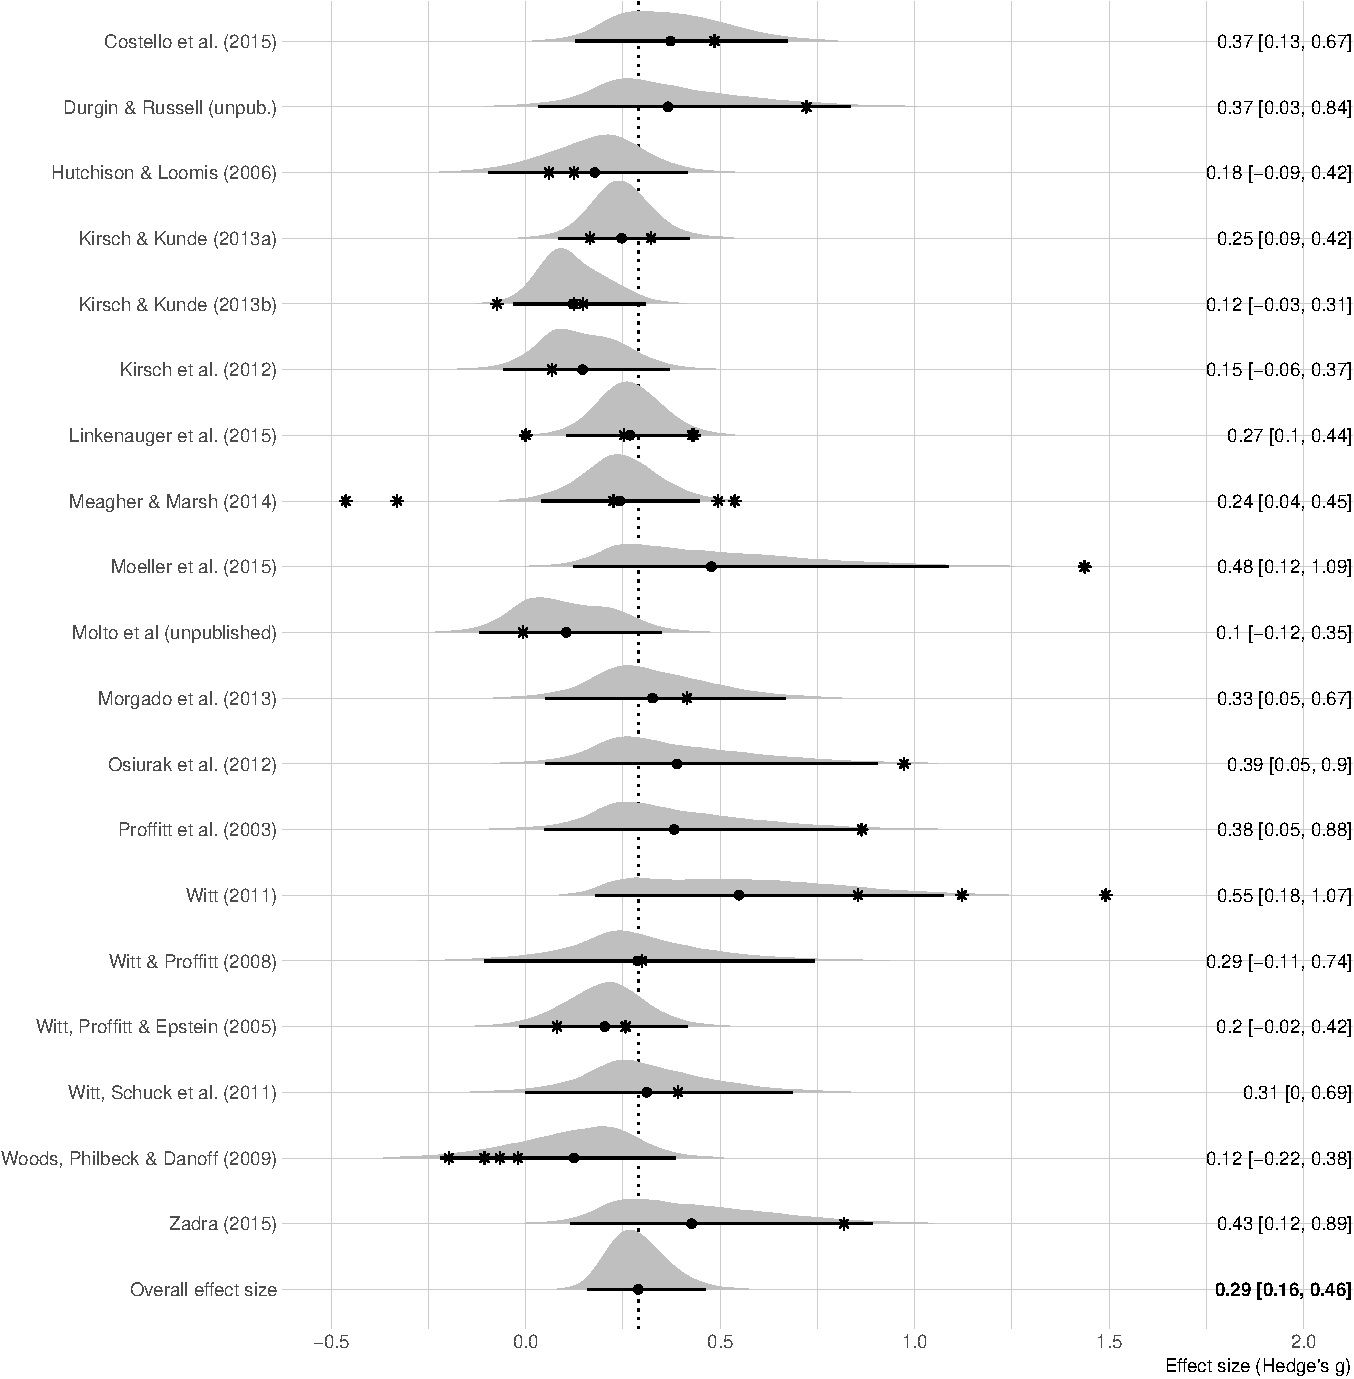
\includegraphics{supplementary_materials_files/figure-latex/forest-1.pdf}
\caption{\label{fig:forest}Forest plot of effect sizes. The densities represent the estimation of the model: the posterior distribution, along with its mean and 95\% credible interval. Raw data (for each experiment) are represented by the stars.}
\end{figure}

\hypertarget{estimation-by-constraint-manipulation}{%
\subsection{Estimation by constraint manipulation}\label{estimation-by-constraint-manipulation}}

We previously provided an estimate of the global effect size of action constraint on distance perception. Below, we estimate the effect size based on the action constraint manipulation by including \texttt{manipulation} as a categorical predictor in the model. We have three categories of manipulation that are: tool-use, weight, and effort. In this model the intercept represents the average effect size corresponding to the \texttt{Effort} manipulation, and the \(\beta\)s for \texttt{Tool-use} and \texttt{Weight} represent deviations from this condition.

\begin{Shaded}
\begin{Highlighting}[]
\NormalTok{data.constraint <-}\StringTok{ }\NormalTok{data }\OperatorTok\StringTok{ }\KeywordTok{filter}\NormalTok{(manipulation }\OperatorTok{!=}\StringTok{ "other"}\NormalTok{)}

\NormalTok{prior2 <-}\StringTok{ }\KeywordTok{c}\NormalTok{(}
    \KeywordTok{prior}\NormalTok{(}\KeywordTok{normal}\NormalTok{(}\DecValTok{0}\NormalTok{, }\DecValTok{1}\NormalTok{), }\DataTypeTok{coef =} \StringTok{"intercept"}\NormalTok{),}
    \KeywordTok{prior}\NormalTok{(}\KeywordTok{normal}\NormalTok{(}\DecValTok{0}\NormalTok{, }\DecValTok{1}\NormalTok{), }\DataTypeTok{class =}\NormalTok{ b),}
    \KeywordTok{prior}\NormalTok{(}\KeywordTok{cauchy}\NormalTok{(}\DecValTok{0}\NormalTok{, }\FloatTok{0.1}\NormalTok{), }\DataTypeTok{class =}\NormalTok{ sd)}
\NormalTok{    )}

\NormalTok{bmod_manip <-}\StringTok{ }\KeywordTok{brm}\NormalTok{(}
\NormalTok{    g }\OperatorTok{|}\StringTok{ }\KeywordTok{se}\NormalTok{(}\KeywordTok{sqrt}\NormalTok{(vi) ) }\OperatorTok{~}\StringTok{ }\DecValTok{0} \OperatorTok{+}\StringTok{ }\NormalTok{intercept }\OperatorTok{+}\StringTok{ }\NormalTok{manipulation }\OperatorTok{+}\StringTok{ }\NormalTok{(}\DecValTok{1}\OperatorTok{|}\NormalTok{article) }\OperatorTok{+}\StringTok{ }\NormalTok{(}\DecValTok{1}\OperatorTok{|}\NormalTok{study),}
    \DataTypeTok{data =}\NormalTok{ data,}
    \DataTypeTok{prior =}\NormalTok{ prior2,}
    \DataTypeTok{sample_prior =} \OtherTok{TRUE}\NormalTok{,}
    \DataTypeTok{warmup =} \DecValTok{5000}\NormalTok{,}
    \DataTypeTok{iter =} \DecValTok{20000}\NormalTok{,}
    \DataTypeTok{cores =}\NormalTok{ parallel}\OperatorTok{::}\KeywordTok{detectCores}\NormalTok{(),}
    \DataTypeTok{control =} \KeywordTok{list}\NormalTok{(}\DataTypeTok{adapt_delta =} \FloatTok{.99}\NormalTok{)}
\NormalTok{    )}
\end{Highlighting}
\end{Shaded}

Below we retrieve samples from the posterior distribution using the \texttt{posterior\_samples()} function. Then, we can use these posterior samples to compare each pair of conditions.

\begin{Shaded}
\begin{Highlighting}[]
\CommentTok{# retrieving the posterior samples}
\NormalTok{post_manip <-}\StringTok{ }\KeywordTok{posterior_samples}\NormalTok{(bmod_manip, }\DataTypeTok{pars =} \StringTok{"^b_"}\NormalTok{)}

\CommentTok{# difference between effort and tool-use}
\NormalTok{contrast1 <-}\StringTok{ }\NormalTok{post_manip[, }\DecValTok{1}\NormalTok{]  }\OperatorTok{-}\StringTok{ }\NormalTok{(post_manip[, }\DecValTok{1}\NormalTok{] }\OperatorTok{+}\StringTok{ }\NormalTok{post_manip[, }\DecValTok{2}\NormalTok{])}

\CommentTok{# difference between effort and weight}
\NormalTok{contrast2 <-}\StringTok{ }\NormalTok{post_manip[, }\DecValTok{1}\NormalTok{]  }\OperatorTok{-}\StringTok{ }\NormalTok{(post_manip[, }\DecValTok{1}\NormalTok{] }\OperatorTok{+}\StringTok{ }\NormalTok{post_manip[, }\DecValTok{3}\NormalTok{])}

\CommentTok{# difference between tool-use and weight}
\NormalTok{contrast3 <-}\StringTok{ }\NormalTok{(post_manip[, }\DecValTok{1}\NormalTok{] }\OperatorTok{+}\StringTok{ }\NormalTok{post_manip[, }\DecValTok{2}\NormalTok{]) }\OperatorTok{-}\StringTok{ }\NormalTok{(post_manip[, }\DecValTok{1}\NormalTok{] }\OperatorTok{+}\StringTok{ }\NormalTok{post_manip[, }\DecValTok{3}\NormalTok{])}
\end{Highlighting}
\end{Shaded}

We then compute Bayes factors for each contrast using the \texttt{hypothesis()} method. This analysis reveals moderate evidence for an absence of difference between \texttt{Tool-use} and \texttt{Weight} (\(\beta\) = 0.27, 95\% CrI {[}-0.23, 0.77, \(BF_{01}\) = 3.10), moderate evidence for an absence of difference between \texttt{Effort} and \texttt{Weight} (\(\beta\) = 0.19, 95\% CrI {[}-0.26, 0.65, \(BF_{01}\) = 3.16), and moderate evidence for an absence of difference between \texttt{Effort} and \texttt{Tool-use} (\(\beta\) = -0.07, 95\% CrI {[}-0.43, 0.30, \(BF_{01}\) = 5.24). We also test the null hypothesis for each constraint manipulation. This reveals moderate evidence for the hypothesis of no effect of weight manipulation (\(\beta\) = 0.13, 95\% CrI {[}-0.26, 0.55{]}, \(BF_{01}\) = 6.16). However, this analysis also reveals moderate to strong evidence for an effect of the AC manipulation (tool-use: \(BF_{10}\) = 3.81 and effort: \(BF_{10}\) = 10.45).

\begin{figure}[H]

{\centering 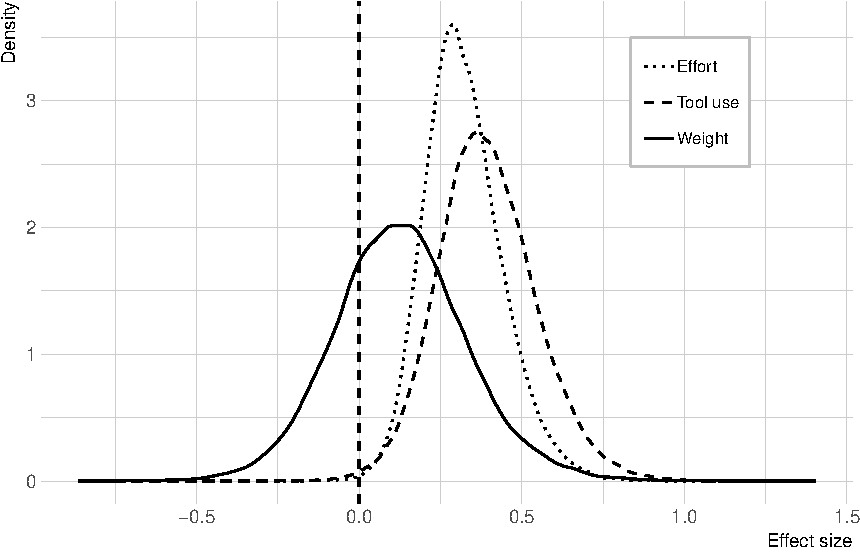
\includegraphics[width=0.75\linewidth]{supplementary_materials_files/figure-latex/unnamed-chunk-12-1} 

}

\caption{Posterior distribution of effect size by constraint manipulation.}\label{fig:unnamed-chunk-12}
\end{figure}

\hypertarget{moderators-analyses}{%
\section{Moderators analyses}\label{moderators-analyses}}

We then fit one model by moderator (meta-regression models) using contrast codes for the research \texttt{design}, the \texttt{motor} intention, and \texttt{space}.

\begin{Shaded}
\begin{Highlighting}[]
\CommentTok{# removing "size" measure}
\NormalTok{data.measure <-}\StringTok{ }\NormalTok{data.m }\OperatorTok\StringTok{ }\KeywordTok{filter}\NormalTok{(Measure }\OperatorTok{!=}\StringTok{ "Size"}\NormalTok{)}

\CommentTok{# contrast coding the moderators}
\NormalTok{data}\OperatorTok{$}\NormalTok{design.c <-}\StringTok{ }\KeywordTok{ifelse}\NormalTok{(data}\OperatorTok{$}\NormalTok{Design }\OperatorTok{==}\StringTok{ }\DecValTok{0}\NormalTok{, }\FloatTok{-0.5}\NormalTok{, }\FloatTok{0.5}\NormalTok{)}
\NormalTok{data.m}\OperatorTok{$}\NormalTok{motor.c <-}\StringTok{ }\KeywordTok{ifelse}\NormalTok{(data.m}\OperatorTok{$}\NormalTok{motor_i }\OperatorTok{==}\StringTok{ }\DecValTok{0}\NormalTok{, }\FloatTok{-0.5}\NormalTok{, }\FloatTok{0.5}\NormalTok{)}
\NormalTok{data}\OperatorTok{$}\NormalTok{space.c <-}\StringTok{ }\KeywordTok{ifelse}\NormalTok{(data}\OperatorTok{$}\NormalTok{space }\OperatorTok{==}\StringTok{ "proche"}\NormalTok{, }\FloatTok{-0.5}\NormalTok{, }\FloatTok{0.5}\NormalTok{)}
\end{Highlighting}
\end{Shaded}

\hypertarget{research-design}{%
\subsection{Research design}\label{research-design}}

We fit a new model including \texttt{design} as a contrast-coded (-0.5, 0.5) predictor and assign it a midly informative normal prior.

\begin{Shaded}
\begin{Highlighting}[]
\NormalTok{bmod_design <-}\StringTok{ }\KeywordTok{brm}\NormalTok{(}
\NormalTok{    g }\OperatorTok{|}\StringTok{ }\KeywordTok{se}\NormalTok{(}\KeywordTok{sqrt}\NormalTok{(vi) ) }\OperatorTok{~}\StringTok{ }\DecValTok{0} \OperatorTok{+}\StringTok{ }\NormalTok{intercept }\OperatorTok{+}\StringTok{ }\NormalTok{design.c }\OperatorTok{+}\StringTok{ }\NormalTok{(}\DecValTok{1}\OperatorTok{|}\NormalTok{article) }\OperatorTok{+}\StringTok{ }\NormalTok{(}\DecValTok{1}\OperatorTok{|}\NormalTok{study),}
    \DataTypeTok{data =}\NormalTok{ data,}
    \DataTypeTok{prior =}\NormalTok{ prior2,}
    \DataTypeTok{sample_prior =} \OtherTok{FALSE}\NormalTok{,}
    \DataTypeTok{save_all_pars =} \OtherTok{TRUE}\NormalTok{,}
    \DataTypeTok{chains =} \DecValTok{4}\NormalTok{,}
    \DataTypeTok{warmup =} \DecValTok{5000}\NormalTok{,}
    \DataTypeTok{iter =} \DecValTok{20000}\NormalTok{,}
    \DataTypeTok{cores =}\NormalTok{ parallel}\OperatorTok{::}\KeywordTok{detectCores}\NormalTok{(),}
    \DataTypeTok{control =} \KeywordTok{list}\NormalTok{(}\DataTypeTok{adapt_delta =} \FloatTok{.99}\NormalTok{)}
\NormalTok{    )}
\end{Highlighting}
\end{Shaded}

Estimations from this model can be retrieved using the \texttt{tidy()} function, as previously.

\begin{Shaded}
\begin{Highlighting}[]
\NormalTok{(bmod_design_est <-}\StringTok{ }\KeywordTok{tidy}\NormalTok{(bmod_design, }\DataTypeTok{parameters =} \KeywordTok{c}\NormalTok{(}\StringTok{"^b_"}\NormalTok{, }\StringTok{"^sd_"}\NormalTok{), }\DataTypeTok{prob =} \FloatTok{0.95}\NormalTok{) )}
\end{Highlighting}
\end{Shaded}

\begin{verbatim}
##                    term   estimate  std.error       lower       upper
## 1           b_intercept  0.3365955 0.07679124  0.20055317 0.502501136
## 2            b_design.c -0.2607505 0.13759405 -0.54082671 0.005648886
## 3 sd_article__Intercept  0.1723962 0.09069850  0.01512193 0.365961446
## 4   sd_study__Intercept  0.1096473 0.05503013  0.01658359 0.233728248
\end{verbatim}

We can test the hypothesis of no difference between the two conditions following the same strategy as previously by comparing the previous model (\texttt{bmod\_design}) to the intercept-only model.

\begin{Shaded}
\begin{Highlighting}[]
\NormalTok{bf_design <-}\StringTok{ }\KeywordTok{bayes_factor}\NormalTok{(}
\NormalTok{    bmod1, bmod_design,}
    \DataTypeTok{repetitions =} \FloatTok{1e2}\NormalTok{, }\DataTypeTok{cores =}\NormalTok{ parallel}\OperatorTok{::}\KeywordTok{detectCores}\NormalTok{()}
\NormalTok{    )}
\end{Highlighting}
\end{Shaded}

There is only anecdotal evidence for an absence of difference between the two conditions (\(\beta\) = -0.26, 95\% CrI {[}-0.54, 0.01{]}, \(BF_{01}\) = 1.04).

\hypertarget{measures}{%
\subsection{Measures}\label{measures}}

We then fit a second model, including \texttt{measures} as a categorical predictor. One advantage of the Bayesian approach is that we can compare conditions (i.e., the different levels of the \texttt{measure} factor) directly from the joint posterior distribution by computing the posterior distribution of the difference.

\begin{Shaded}
\begin{Highlighting}[]
\NormalTok{bmod_measure <-}\StringTok{ }\KeywordTok{brm}\NormalTok{(}
\NormalTok{    g }\OperatorTok{|}\StringTok{ }\KeywordTok{se}\NormalTok{(}\KeywordTok{sqrt}\NormalTok{(vi) ) }\OperatorTok{~}\StringTok{ }\DecValTok{0} \OperatorTok{+}\StringTok{ }\NormalTok{intercept }\OperatorTok{+}\StringTok{ }\NormalTok{Measure }\OperatorTok{+}\StringTok{ }\NormalTok{(}\DecValTok{1}\OperatorTok{|}\NormalTok{article) }\OperatorTok{+}\StringTok{ }\NormalTok{(}\DecValTok{1}\OperatorTok{|}\NormalTok{study),}
    \DataTypeTok{data =}\NormalTok{ data.measure,}
    \DataTypeTok{prior =}\NormalTok{ prior2,}
    \DataTypeTok{sample_prior =} \OtherTok{TRUE}\NormalTok{,}
    \DataTypeTok{warmup =} \DecValTok{5000}\NormalTok{,}
    \DataTypeTok{iter =} \DecValTok{20000}\NormalTok{,}
    \DataTypeTok{cores =}\NormalTok{ parallel}\OperatorTok{::}\KeywordTok{detectCores}\NormalTok{(),}
    \DataTypeTok{control =} \KeywordTok{list}\NormalTok{(}\DataTypeTok{adapt_delta =} \FloatTok{.99}\NormalTok{)}
\NormalTok{    )}
\end{Highlighting}
\end{Shaded}

\begin{Shaded}
\begin{Highlighting}[]
\NormalTok{(bmod_measure_est <-}\StringTok{ }\KeywordTok{tidy}\NormalTok{(bmod_measure, }\DataTypeTok{parameters =} \KeywordTok{c}\NormalTok{(}\StringTok{"^b_"}\NormalTok{, }\StringTok{"^sd_"}\NormalTok{), }\DataTypeTok{prob =} \FloatTok{0.95}\NormalTok{) )}
\end{Highlighting}
\end{Shaded}

\begin{verbatim}
##                    term   estimate  std.error        lower     upper
## 1           b_intercept 0.21248606 0.15262114 -0.084067579 0.5172644
## 2       b_MeasureVerbal 0.02308512 0.16067934 -0.289434887 0.3446412
## 3           b_MeasureVm 0.08985221 0.16358243 -0.219500987 0.4223592
## 4 sd_article__Intercept 0.16751815 0.11033420  0.007429043 0.4075180
## 5   sd_study__Intercept 0.19733426 0.07550467  0.060562809 0.3552492
\end{verbatim}

In this model the intercept represents the condition \texttt{MeasureAction}, and the \(\beta\)s for \texttt{MeasureVerbal} and \texttt{MeasureVm} represent deviations from this condition. Below we retrieve samples from the posterior distribution using the \texttt{posterior\_samples()} function.

\begin{Shaded}
\begin{Highlighting}[]
\NormalTok{post <-}\StringTok{ }\KeywordTok{posterior_samples}\NormalTok{(bmod_measure, }\DataTypeTok{pars =} \StringTok{"^b_"}\NormalTok{)}
\KeywordTok{head}\NormalTok{(post)}
\end{Highlighting}
\end{Shaded}

\begin{verbatim}
##   b_intercept b_MeasureVerbal b_MeasureVm
## 1  0.29010040     -0.03829614  0.06234317
## 2  0.01358407     -0.05568620  0.26858131
## 3  0.22265255     -0.02671598 -0.08573913
## 4 -0.12663250      0.36230912  0.34300500
## 5  0.25094556     -0.05162500  0.23697637
## 6  0.25326721      0.06969551  0.23901304
\end{verbatim}

Then, we can use these posterior samples to compare the conditions with each other.

\begin{Shaded}
\begin{Highlighting}[]
\CommentTok{# difference between verbal and vm}
\NormalTok{c1 <-}\StringTok{ }\NormalTok{(post[, }\DecValTok{1}\NormalTok{] }\OperatorTok{+}\StringTok{ }\NormalTok{post[, }\DecValTok{2}\NormalTok{]) }\OperatorTok{-}\StringTok{ }\NormalTok{(post[, }\DecValTok{1}\NormalTok{] }\OperatorTok{+}\StringTok{ }\NormalTok{post[, }\DecValTok{3}\NormalTok{])}

\CommentTok{# difference between verbal and action}
\NormalTok{c2 <-}\StringTok{ }\NormalTok{(post[, }\DecValTok{1}\NormalTok{] }\OperatorTok{+}\StringTok{ }\NormalTok{post[, }\DecValTok{2}\NormalTok{]) }\OperatorTok{-}\StringTok{ }\NormalTok{post[, }\DecValTok{1}\NormalTok{]}

\CommentTok{# difference between action and vm}
\NormalTok{c3 <-}\StringTok{ }\NormalTok{post[, }\DecValTok{1}\NormalTok{] }\OperatorTok{-}\StringTok{ }\NormalTok{(post[, }\DecValTok{1}\NormalTok{] }\OperatorTok{+}\StringTok{ }\NormalTok{post[, }\DecValTok{3}\NormalTok{])}
\end{Highlighting}
\end{Shaded}

We can plot the posterior distribution corresponding to each \emph{contrast}, using the \texttt{BEST} package (Kruschke \& Meredith, 2017). Below, we plot the contrast \texttt{c1}, which represents the comparison of the \texttt{verbal} and \texttt{vm} conditions.

\begin{Shaded}
\begin{Highlighting}[]
\KeywordTok{library}\NormalTok{(BEST)}
\KeywordTok{par}\NormalTok{(}\DataTypeTok{cex =} \FloatTok{0.75}\NormalTok{, }\DataTypeTok{cex.lab =} \FloatTok{0.75}\NormalTok{)}
\KeywordTok{plotPost}\NormalTok{(c1, }\DataTypeTok{credMass =} \FloatTok{0.95}\NormalTok{, }\DataTypeTok{compVal =} \DecValTok{0}\NormalTok{, }\DataTypeTok{col =} \StringTok{"#b3cde0"}\NormalTok{)}
\end{Highlighting}
\end{Shaded}

\begin{figure}[H]

{\centering 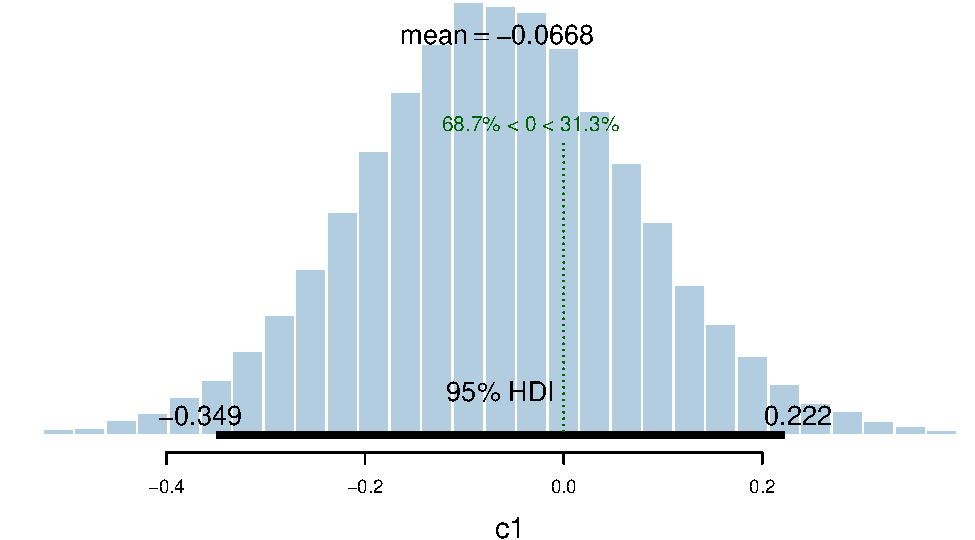
\includegraphics[width=0.75\linewidth]{supplementary_materials_files/figure-latex/unnamed-chunk-23-1} 

}

\caption{Posterior distribution of the difference between verbal and vm.}\label{fig:unnamed-chunk-23}
\end{figure}

We can then compute the Bayes Factor for this difference using the \texttt{hypothesis()} function.

\begin{Shaded}
\begin{Highlighting}[]
\KeywordTok{hypothesis}\NormalTok{(}
\NormalTok{    bmod_measure, }\StringTok{"(intercept + MeasureVerbal) = (intercept + MeasureVm)"}\NormalTok{,}
    \DataTypeTok{seed =} \DecValTok{123}
\NormalTok{    )}
\end{Highlighting}
\end{Shaded}

\begin{verbatim}
## Hypothesis Tests for class b:
##                 Hypothesis Estimate Est.Error CI.Lower CI.Upper Evid.Ratio
## 1 ((intercept+Measu... = 0    -0.07      0.14    -0.35     0.22       9.08
##   Post.Prob Star
## 1       0.9     
## ---
## '*': The expected value under the hypothesis lies outside the 95%-CI.
## Posterior probabilities of point hypotheses assume equal prior probabilities.
\end{verbatim}

We can then follow the same strategy for the two other contrasts, \texttt{c2} and \texttt{c3}, by plotting the posterior distribution of the difference between the two conditions.

\begin{Shaded}
\begin{Highlighting}[]
\KeywordTok{par}\NormalTok{(}\DataTypeTok{cex =} \FloatTok{0.75}\NormalTok{, }\DataTypeTok{cex.lab =} \FloatTok{0.75}\NormalTok{)}
\KeywordTok{plotPost}\NormalTok{(c2, }\DataTypeTok{credMass =} \FloatTok{0.95}\NormalTok{, }\DataTypeTok{compVal =} \DecValTok{0}\NormalTok{, }\DataTypeTok{col =} \StringTok{"#b3cde0"}\NormalTok{)}
\end{Highlighting}
\end{Shaded}

\begin{figure}[H]

{\centering 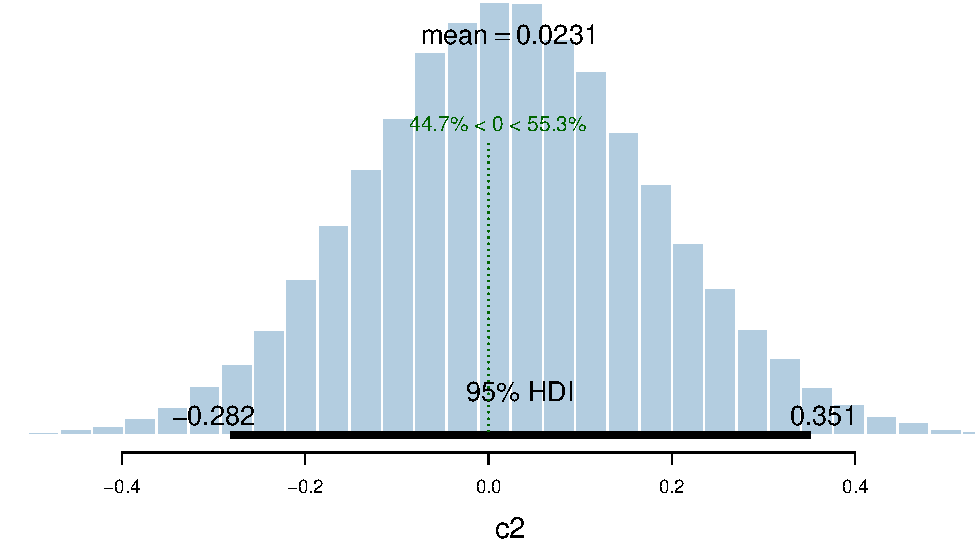
\includegraphics[width=0.75\linewidth]{supplementary_materials_files/figure-latex/unnamed-chunk-25-1} 

}

\caption{Posterior distribution of the contrast.}\label{fig:unnamed-chunk-251}
\end{figure}

\begin{Shaded}
\begin{Highlighting}[]
\KeywordTok{plotPost}\NormalTok{(c3, }\DataTypeTok{credMass =} \FloatTok{0.95}\NormalTok{, }\DataTypeTok{compVal =} \DecValTok{0}\NormalTok{, }\DataTypeTok{col =} \StringTok{"#b3cde0"}\NormalTok{)}
\end{Highlighting}
\end{Shaded}

\begin{figure}[H]

{\centering 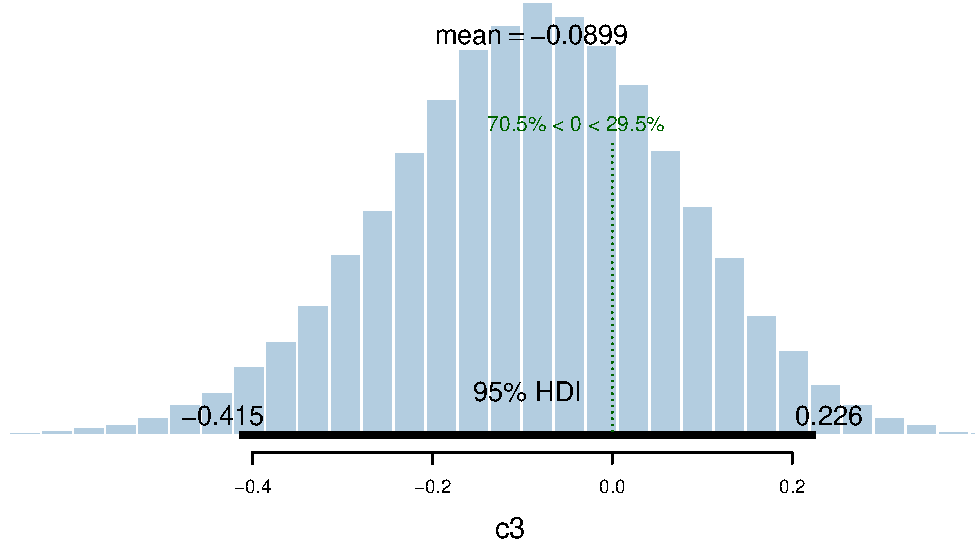
\includegraphics[width=0.75\linewidth]{supplementary_materials_files/figure-latex/unnamed-chunk-25-2} 

}

\caption{Posterior distribution of the contrast.}\label{fig:unnamed-chunk-252}
\end{figure}

We then compute the Bayes Factor for these differences using the \texttt{hypothesis()} function, as previously.

\begin{Shaded}
\begin{Highlighting}[]
\KeywordTok{hypothesis}\NormalTok{(}
\NormalTok{    bmod_measure, }\StringTok{"(intercept) = (intercept + MeasureVerbal)"}\NormalTok{,}
    \DataTypeTok{seed =} \DecValTok{123}
\NormalTok{    )}
\end{Highlighting}
\end{Shaded}

\begin{verbatim}
## Hypothesis Tests for class b:
##                 Hypothesis Estimate Est.Error CI.Lower CI.Upper Evid.Ratio
## 1 ((intercept))-((i... = 0    -0.02      0.16    -0.34     0.29       6.28
##   Post.Prob Star
## 1      0.86     
## ---
## '*': The expected value under the hypothesis lies outside the 95%-CI.
## Posterior probabilities of point hypotheses assume equal prior probabilities.
\end{verbatim}

\begin{Shaded}
\begin{Highlighting}[]
\KeywordTok{hypothesis}\NormalTok{(}
\NormalTok{    bmod_measure, }\StringTok{"(intercept) = (intercept + MeasureVm)"}\NormalTok{,}
    \DataTypeTok{seed =} \DecValTok{123}
\NormalTok{    )}
\end{Highlighting}
\end{Shaded}

\begin{verbatim}
## Hypothesis Tests for class b:
##                 Hypothesis Estimate Est.Error CI.Lower CI.Upper Evid.Ratio
## 1 ((intercept))-((i... = 0    -0.09      0.16    -0.42     0.22       5.55
##   Post.Prob Star
## 1      0.85     
## ---
## '*': The expected value under the hypothesis lies outside the 95%-CI.
## Posterior probabilities of point hypotheses assume equal prior probabilities.
\end{verbatim}

\hypertarget{motor-intention}{%
\subsection{Motor intention}\label{motor-intention}}

As previously, we can fit a new model including \texttt{motor\ intention} as a contrast-coded categorical predictor with a midly informative normal prior.

\begin{Shaded}
\begin{Highlighting}[]
\NormalTok{bmod_motor <-}\StringTok{ }\KeywordTok{brm}\NormalTok{(}
\NormalTok{    g }\OperatorTok{|}\StringTok{ }\KeywordTok{se}\NormalTok{(}\KeywordTok{sqrt}\NormalTok{(vi) ) }\OperatorTok{~}\StringTok{ }\DecValTok{0} \OperatorTok{+}\StringTok{ }\NormalTok{intercept }\OperatorTok{+}\StringTok{ }\NormalTok{motor.c }\OperatorTok{+}\StringTok{ }\NormalTok{(}\DecValTok{1}\OperatorTok{|}\NormalTok{article) }\OperatorTok{+}\StringTok{ }\NormalTok{(}\DecValTok{1}\OperatorTok{|}\NormalTok{study),}
    \DataTypeTok{data =}\NormalTok{ data.m,}
    \DataTypeTok{prior =}\NormalTok{ prior2,}
    \DataTypeTok{save_all_pars =} \OtherTok{TRUE}\NormalTok{,}
    \DataTypeTok{chains =} \DecValTok{4}\NormalTok{,}
    \DataTypeTok{warmup =} \DecValTok{5000}\NormalTok{,}
    \DataTypeTok{iter =} \DecValTok{20000}\NormalTok{,}
    \DataTypeTok{cores =}\NormalTok{ parallel}\OperatorTok{::}\KeywordTok{detectCores}\NormalTok{(),}
    \DataTypeTok{control =} \KeywordTok{list}\NormalTok{(}\DataTypeTok{adapt_delta =} \FloatTok{.99}\NormalTok{)}
\NormalTok{    )}
\end{Highlighting}
\end{Shaded}

\begin{Shaded}
\begin{Highlighting}[]
\NormalTok{(bmod_motor_est <-}\StringTok{ }\KeywordTok{tidy}\NormalTok{(bmod_motor, }\DataTypeTok{parameters =} \KeywordTok{c}\NormalTok{(}\StringTok{"^b_"}\NormalTok{, }\StringTok{"^sd_"}\NormalTok{), }\DataTypeTok{prob =} \FloatTok{0.95}\NormalTok{) )}
\end{Highlighting}
\end{Shaded}

\begin{verbatim}
##                    term   estimate  std.error       lower     upper
## 1           b_intercept 0.25538755 0.09374274  0.08907247 0.4562718
## 2             b_motor.c 0.06930065 0.14941719 -0.23000842 0.3606807
## 3 sd_article__Intercept 0.20345941 0.11063563  0.01432974 0.4365166
## 4   sd_study__Intercept 0.15321818 0.06982372  0.03348667 0.3031598
\end{verbatim}

We can then test whether the difference between the two conditions is equal to zero, following the same strategy as previously.

\begin{Shaded}
\begin{Highlighting}[]
\NormalTok{bf_motor <-}\StringTok{ }\KeywordTok{bayes_factor}\NormalTok{(}
\NormalTok{    bmod1, bmod_motor,}
    \DataTypeTok{repetitions =} \FloatTok{1e2}\NormalTok{, }\DataTypeTok{cores =}\NormalTok{ parallel}\OperatorTok{::}\KeywordTok{detectCores}\NormalTok{()}
\NormalTok{    )}
\end{Highlighting}
\end{Shaded}

There is strong evidence for an absence of difference between the two conditions (\(\beta\) = 0.07, 95\% CrI {[}-0.23, 0.36{]}, \(BF_{01}\) = 10,096.54).

\hypertarget{distance-from-target}{%
\subsection{Distance from target}\label{distance-from-target}}

We fit below a new model including target presence (\texttt{space.c}) as a contrast-coded (-0.5, 0.5) categorical predictor, and assign it a midly informative normal prior.

\begin{Shaded}
\begin{Highlighting}[]
\NormalTok{bmod_space <-}\StringTok{ }\KeywordTok{brm}\NormalTok{(}
\NormalTok{    g }\OperatorTok{|}\StringTok{ }\KeywordTok{se}\NormalTok{(}\KeywordTok{sqrt}\NormalTok{(vi) ) }\OperatorTok{~}\StringTok{ }\DecValTok{0} \OperatorTok{+}\StringTok{ }\NormalTok{intercept }\OperatorTok{+}\StringTok{ }\NormalTok{space.c }\OperatorTok{+}\StringTok{ }\NormalTok{(}\DecValTok{1}\OperatorTok{|}\NormalTok{article) }\OperatorTok{+}\StringTok{ }\NormalTok{(}\DecValTok{1}\OperatorTok{|}\NormalTok{study),}
    \DataTypeTok{data =}\NormalTok{ data,}
    \DataTypeTok{prior =}\NormalTok{ prior2,}
    \DataTypeTok{sample_prior =} \OtherTok{FALSE}\NormalTok{,}
    \DataTypeTok{save_all_pars =} \OtherTok{TRUE}\NormalTok{,}
    \DataTypeTok{chains =} \DecValTok{4}\NormalTok{,}
    \DataTypeTok{warmup =} \DecValTok{5000}\NormalTok{,}
    \DataTypeTok{iter =} \DecValTok{20000}\NormalTok{,}
    \DataTypeTok{cores =}\NormalTok{ parallel}\OperatorTok{::}\KeywordTok{detectCores}\NormalTok{(),}
    \DataTypeTok{control =} \KeywordTok{list}\NormalTok{(}\DataTypeTok{adapt_delta =} \FloatTok{.99}\NormalTok{)}
\NormalTok{    )}
\end{Highlighting}
\end{Shaded}

Estimations of this model can be retrieved using the \texttt{tidy()} function.

\begin{Shaded}
\begin{Highlighting}[]
\NormalTok{(bmod_space_est <-}\StringTok{ }\KeywordTok{tidy}\NormalTok{(bmod_space, }\DataTypeTok{parameters =} \KeywordTok{c}\NormalTok{(}\StringTok{"^b_"}\NormalTok{, }\StringTok{"^sd_"}\NormalTok{), }\DataTypeTok{prob =} \FloatTok{0.95}\NormalTok{) )}
\end{Highlighting}
\end{Shaded}

\begin{verbatim}
##                    term   estimate  std.error       lower     upper
## 1           b_intercept 0.31425196 0.08593040  0.16586409 0.5037808
## 2             b_space.c 0.09729085 0.15428004 -0.20127676 0.4150503
## 3 sd_article__Intercept 0.20681083 0.10472691  0.01852187 0.4265177
## 4   sd_study__Intercept 0.11866278 0.06073119  0.01946639 0.2573810
\end{verbatim}

We can test whether the difference between the two conditions is equal to zero by computing a Bayes Factor using the \texttt{bayes\_factor()} method.

\begin{Shaded}
\begin{Highlighting}[]
\NormalTok{bf_space <-}\StringTok{ }\KeywordTok{bayes_factor}\NormalTok{(bmod1, bmod_space, }\DataTypeTok{repetitions =} \FloatTok{1e2}\NormalTok{, }\DataTypeTok{cores =}\NormalTok{ parallel}\OperatorTok{::}\KeywordTok{detectCores}\NormalTok{() )}
\end{Highlighting}
\end{Shaded}

There is only anecdotal evidence for an absence of difference between the two conditions (\(\beta\) = 0.10, 95\% CrI {[}-0.20, 0.42{]}, \(BF_{01}\) = 5.71). Below, we plot the marginal posterior distribution of the effect size by condition, for each moderator.

\begin{figure}[H]

{\centering 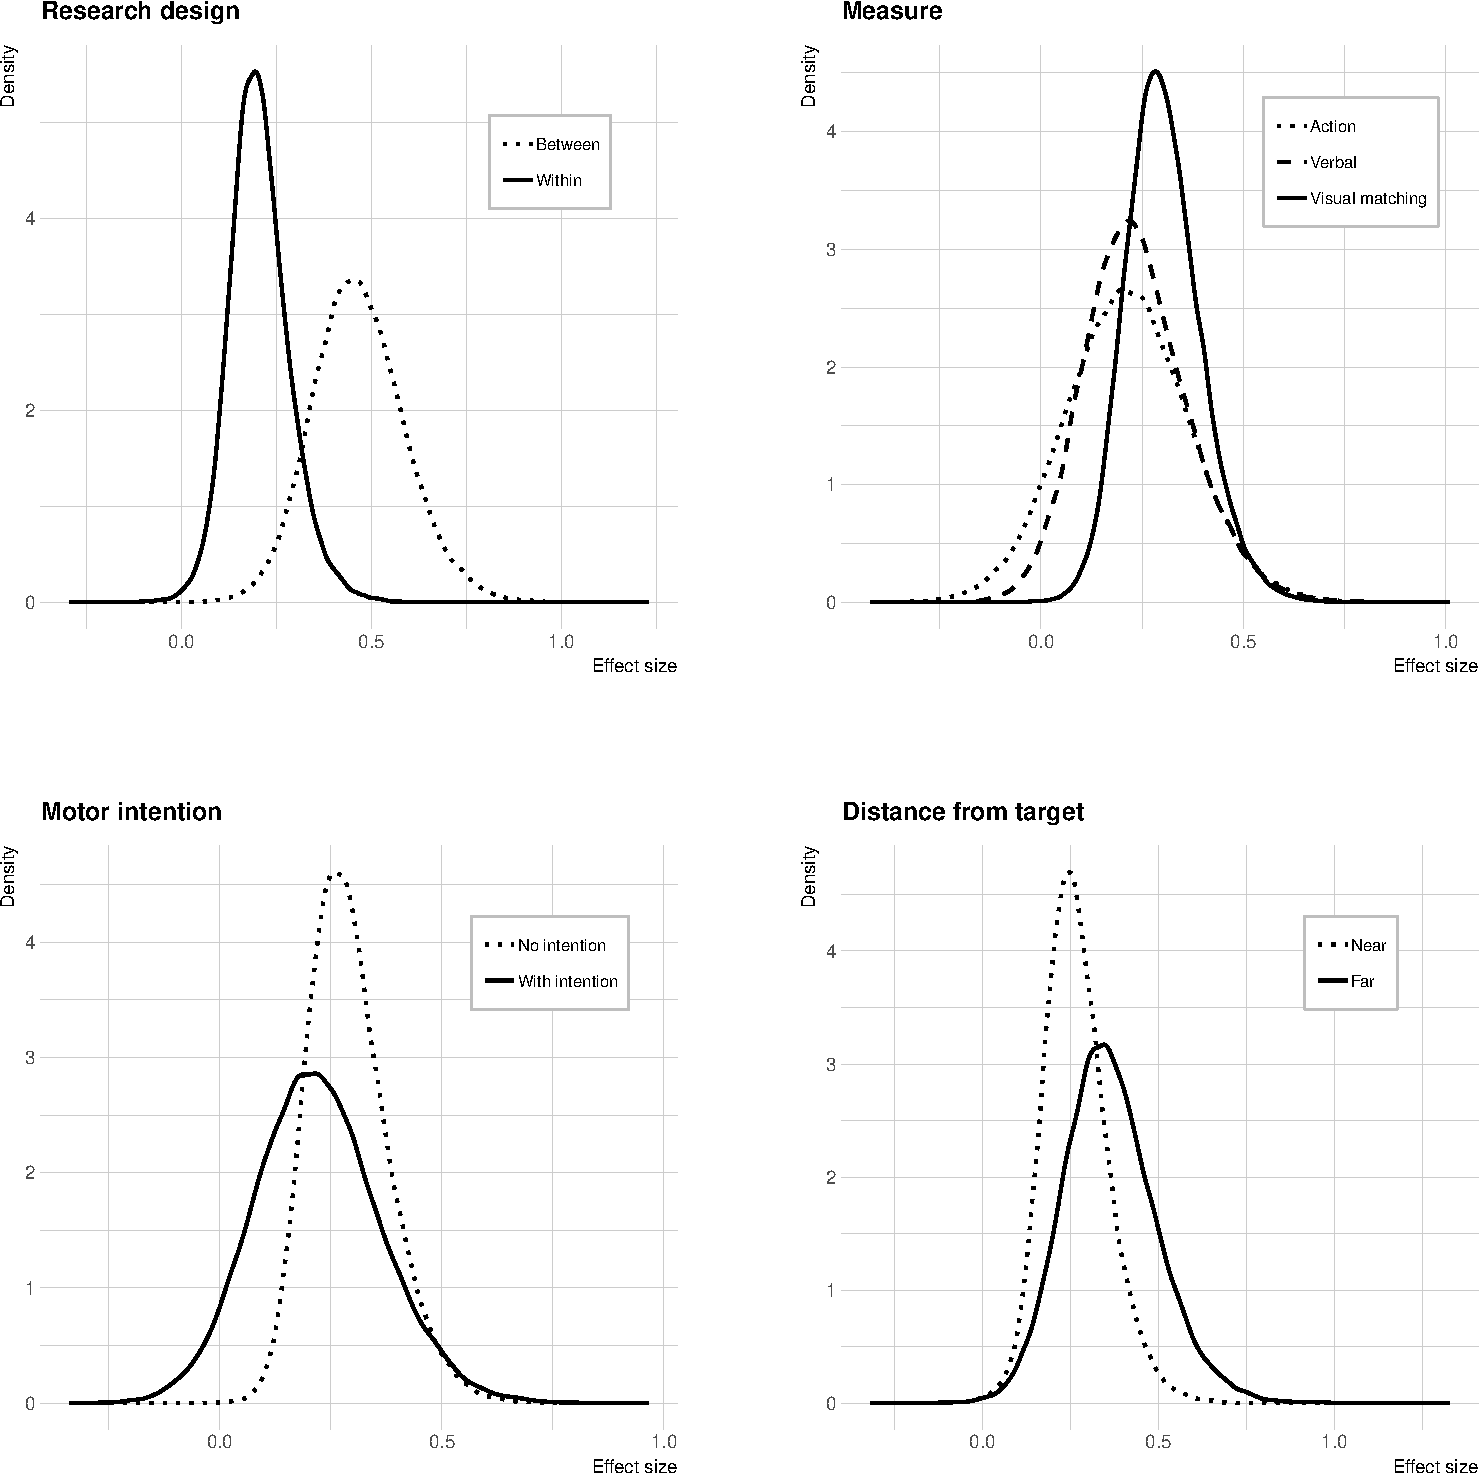
\includegraphics{supplementary_materials_files/figure-latex/unnamed-chunk-36-1} 

}

\caption{Posterior distribution of the effect size by condition.}\label{fig:unnamed-chunk-36}
\end{figure}

\hypertarget{additional-analyses}{%
\section{Additional analyses}\label{additional-analyses}}

\hypertarget{publication-bias}{%
\subsection{Publication bias}\label{publication-bias}}

If there is no publication bias, the funnel plot should look symmetric with outcomes dispersed equally on both sides of the average effect size. However, if studies with null results are missing, the funnel plot might look asymmetric with studies on the left side of the mean estimate missing.

\begin{Shaded}
\begin{Highlighting}[]
\KeywordTok{library}\NormalTok{(metaviz)}
\KeywordTok{library}\NormalTok{(metafor)}

\CommentTok{# create the funnel plot from a metafor model (for convenience)}
\NormalTok{res <-}\StringTok{ }\KeywordTok{rma}\NormalTok{(}\DataTypeTok{yi =}\NormalTok{ g, vi, }\DataTypeTok{data =}\NormalTok{ data, }\DataTypeTok{measure =} \StringTok{"GEN"}\NormalTok{)}

\CommentTok{# customised ggplot2 funnel plot}
\KeywordTok{source}\NormalTok{(}\KeywordTok{here}\NormalTok{(}\StringTok{"code"}\NormalTok{, }\StringTok{"funnel_viz2.R"}\NormalTok{) )}

\KeywordTok{viz_funnel2}\NormalTok{(}
    \DataTypeTok{x =}\NormalTok{ res, }\DataTypeTok{method =} \StringTok{"REML"}\NormalTok{,}
    \DataTypeTok{contours =} \OtherTok{TRUE}\NormalTok{, }\DataTypeTok{sig_contours =} \OtherTok{FALSE}\NormalTok{,}
    \DataTypeTok{contours_col =} \StringTok{"Greys"}\NormalTok{, }\DataTypeTok{xlab =} \StringTok{"Observed outcome"}
\NormalTok{    ) }\OperatorTok{+}
\StringTok{    }\KeywordTok{theme_ipsum}\NormalTok{(}
        \DataTypeTok{base_family =} \StringTok{"Helvetica"}\NormalTok{,}
        \DataTypeTok{base_size =} \DecValTok{10}\NormalTok{, }\DataTypeTok{plot_title_size =} \DecValTok{12}\NormalTok{, }\DataTypeTok{axis_text_size =} \DecValTok{9}
\NormalTok{        )}
\end{Highlighting}
\end{Shaded}

\begin{figure}[H]

{\centering 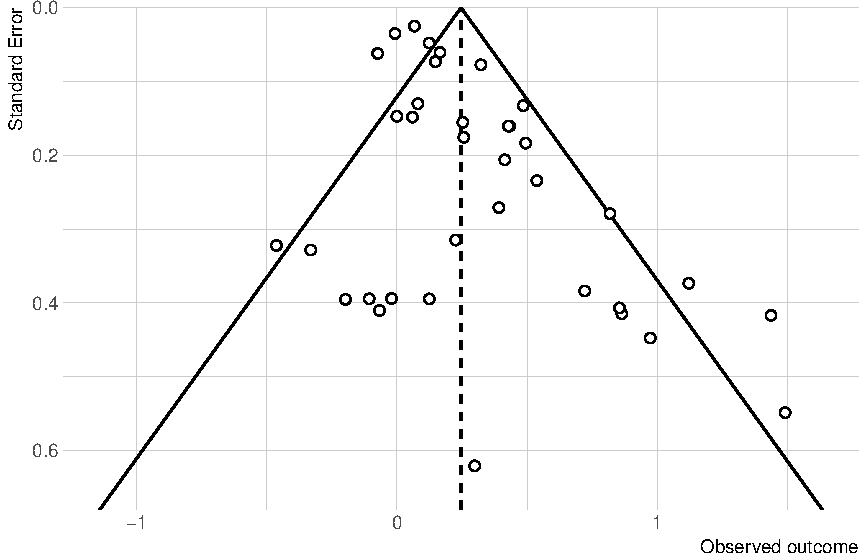
\includegraphics[width=0.75\linewidth]{supplementary_materials_files/figure-latex/funnel1-1} 

}

\caption{Funnel plot with effect sizes on x-axis and standard errors on the y-axis.}\label{fig:funnel1}
\end{figure}

Below, we make a contour-enhanced funnel plot, allowing to distinguish patterns of significance in published studies (Peters, Sutton, Jones, Abrams, \& Rushton, 2008), using the \texttt{metaviz} package (Kossmeier, Tran, \& Voracek, 2018).

\begin{Shaded}
\begin{Highlighting}[]
\KeywordTok{viz_funnel}\NormalTok{(}
    \DataTypeTok{x =}\NormalTok{ res, }\DataTypeTok{method =} \StringTok{"REML"}\NormalTok{,}
    \DataTypeTok{contours =} \OtherTok{FALSE}\NormalTok{, }\DataTypeTok{sig_contours =} \OtherTok{TRUE}\NormalTok{, }\DataTypeTok{detail_level =} \DecValTok{1}\NormalTok{,}
    \DataTypeTok{contours_col =} \StringTok{"Greys"}\NormalTok{,}
    \DataTypeTok{xlab =} \StringTok{"Observed outcome"}
\NormalTok{    ) }\OperatorTok{+}
\StringTok{    }\KeywordTok{geom_vline}\NormalTok{(}\DataTypeTok{xintercept =} \DecValTok{0}\NormalTok{, }\DataTypeTok{linetype =} \DecValTok{2}\NormalTok{) }\OperatorTok{+}
\StringTok{    }\KeywordTok{theme_ipsum}\NormalTok{(}
        \DataTypeTok{base_family =} \StringTok{"Helvetica"}\NormalTok{,}
        \DataTypeTok{base_size =} \DecValTok{10}\NormalTok{, }\DataTypeTok{plot_title_size =} \DecValTok{12}\NormalTok{, }\DataTypeTok{axis_text_size =} \DecValTok{9}
\NormalTok{        )}
\end{Highlighting}
\end{Shaded}

\begin{figure}[H]

{\centering 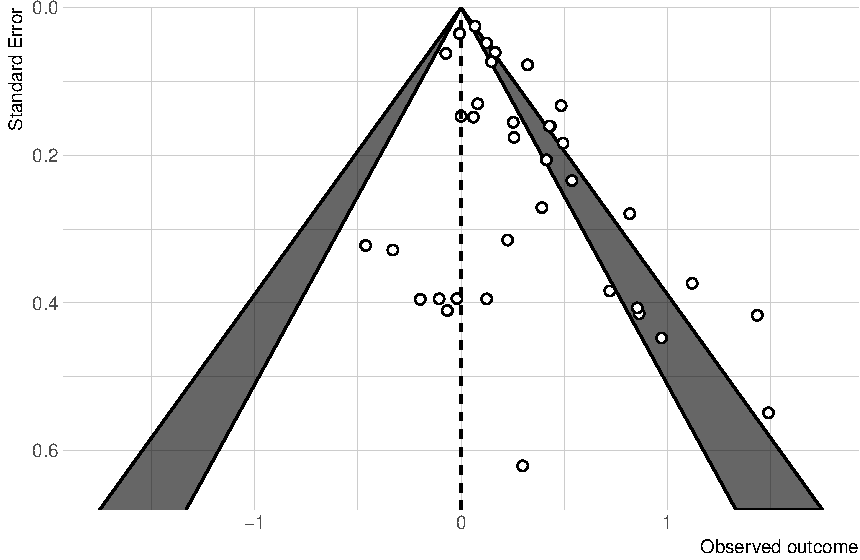
\includegraphics[width=0.75\linewidth]{supplementary_materials_files/figure-latex/funnel2-1} 

}

\caption{Contour-enhanced funnel plot with effect sizes on x-axis and standard errors on the y-axis. Ranges of p-values from the experiments are indicated by the shaded regions. White region inside the funnel corresponds to p-values greater than .05, the gray-shaded region corresponds to p-values between .05 and .01, and the white region outside of the funnel corresponds to p-values below .01.}\label{fig:funnel2}
\end{figure}

\hypertarget{p-curve}{%
\subsection{P-curve}\label{p-curve}}

P-curve analyses test whether a set of p-values supports the existence of an effect. If there is no effect, p-values should be uniformly distributed, whereas if there is an effect, p-values distribution should be right-skewed, with more p-values close to .01 than .05. The observed distribution of p-values from our database is close to a distribution that would be expected with a \emph{true} non-null effect, although it does not differ significantly from the distribution of p-values we would expect for a small effect size and a power of 33\%. Moreover, the uptick of the observed p-curve at p-values of .04 and .05 might indicate data snooping (e.g., p-hacking, QRPs).

\begin{Shaded}
\begin{Highlighting}[]
\KeywordTok{source}\NormalTok{(}\KeywordTok{here}\NormalTok{(}\StringTok{"code"}\NormalTok{, }\StringTok{"pcurve"}\NormalTok{, }\StringTok{"pcurve.R"}\NormalTok{) )}
\NormalTok{knitr}\OperatorTok{::}\KeywordTok{include_graphics}\NormalTok{(}\KeywordTok{here}\NormalTok{(}\StringTok{"code"}\NormalTok{, }\StringTok{"pcurve"}\NormalTok{, }\StringTok{"p_curve.pdf"}\NormalTok{) )}
\end{Highlighting}
\end{Shaded}

\begin{figure}[H]

{\centering 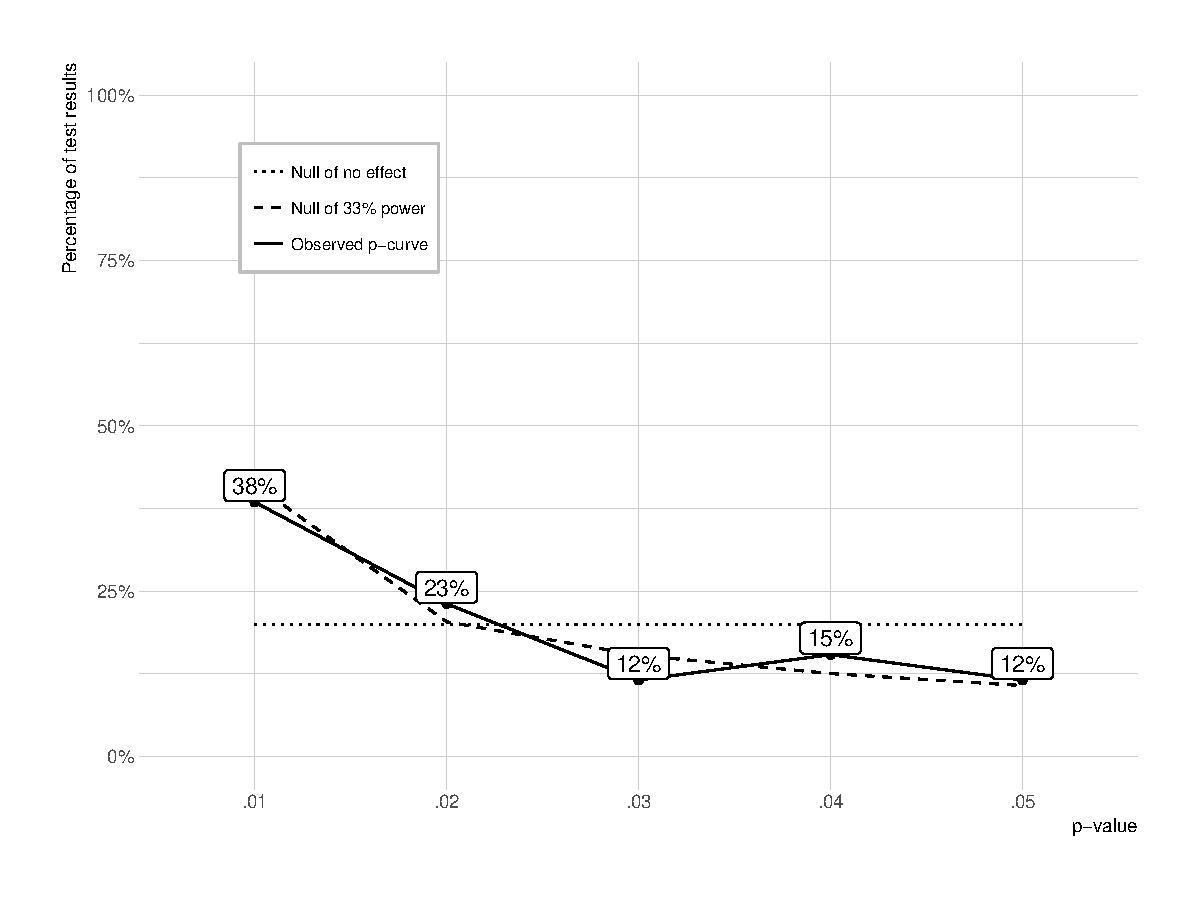
\includegraphics[width=0.75\linewidth]{/Users/Ladislas/Desktop/Academia/projects/submitted/meta_distance_perception/code/pcurve/p_curve} 

}

\caption{P-curve estimation of average power of individual studies: .85, 90\% CI [.70, .94]. The observed p-curve includes 21 statistically significant (p < .05) results of which 17 were inferior to .025. There were 14 additional results entered but excluded from p-curve because they were superior to .05.}\label{fig:pcurve}
\end{figure}

\newpage

\hypertarget{power-analysis}{%
\subsection{Power analysis}\label{power-analysis}}

Below, we illustrate the sample size needed to reach a given level of statistical power according to the AC effects of interest.

\begin{figure}
\centering
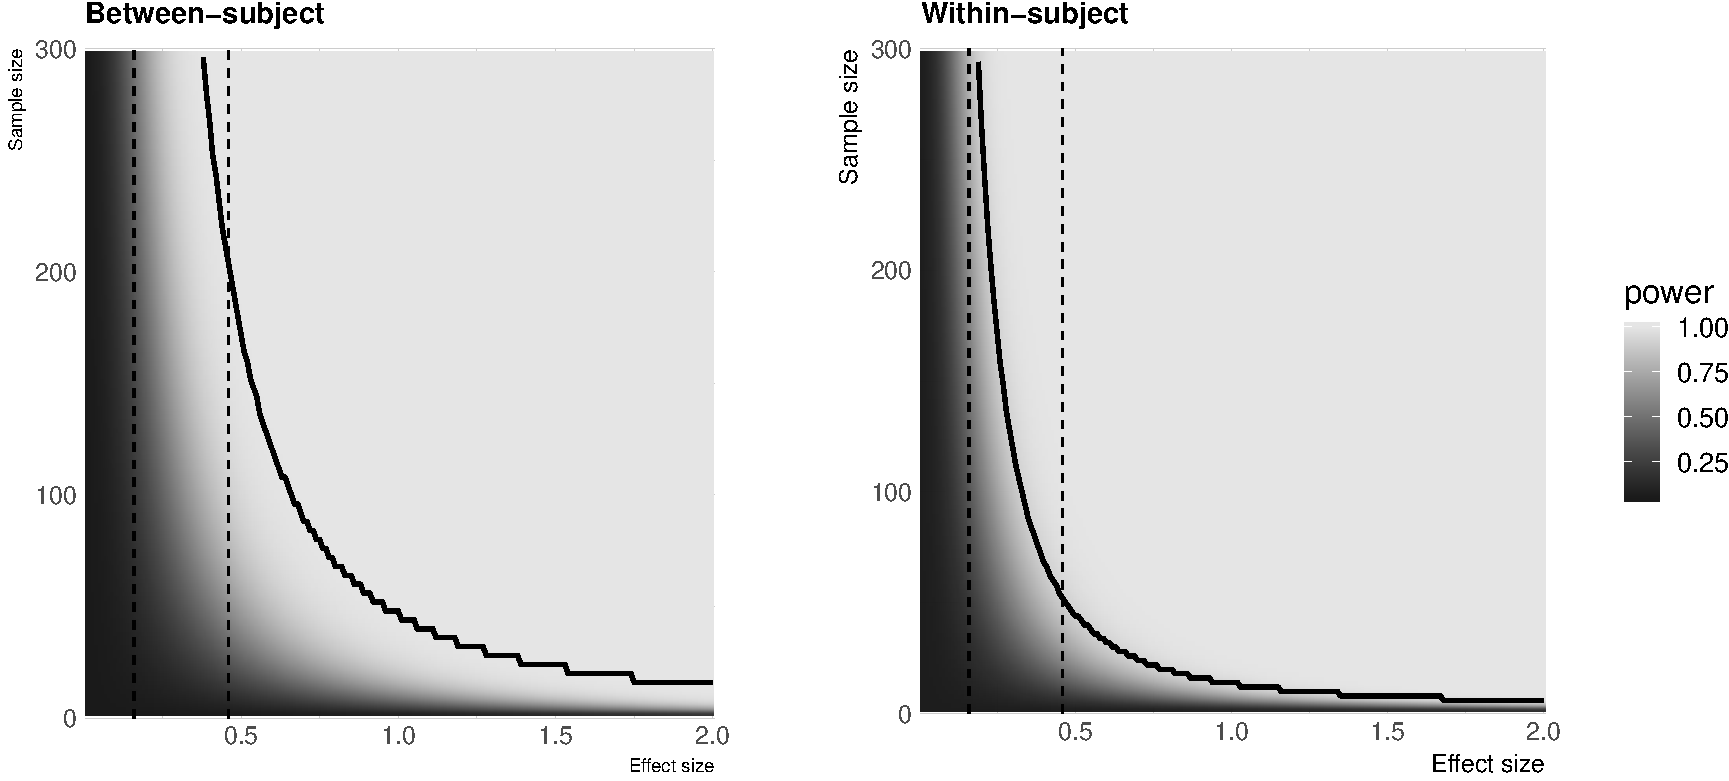
\includegraphics{supplementary_materials_files/figure-latex/power-1.pdf}
\caption{\label{fig:power}Statistical power as a function of sample size, effect size, and research design (left panel: between-subject design; right panel: within-subject design), with a Type 1 error rate (alpha level) fixed at .05. The interval between the dashed lines indicates the 95\% most credible effect sizes as estimated by our model. The black curve corresponds to the recommended power (0.9).}
\end{figure}

\newpage

\hypertarget{session-information}{%
\section{Session information}\label{session-information}}

\begin{Shaded}
\begin{Highlighting}[]
\KeywordTok{sessionInfo}\NormalTok{()}
\end{Highlighting}
\end{Shaded}

\begin{verbatim}
## R version 3.5.3 (2019-03-11)
## Platform: x86_64-apple-darwin15.6.0 (64-bit)
## Running under: macOS Mojave 10.14
## 
## Matrix products: default
## BLAS: /Library/Frameworks/R.framework/Versions/3.5/Resources/lib/libRblas.0.dylib
## LAPACK: /Library/Frameworks/R.framework/Versions/3.5/Resources/lib/libRlapack.dylib
## 
## locale:
## [1] en_US.UTF-8/en_US.UTF-8/en_US.UTF-8/C/en_US.UTF-8/en_US.UTF-8
## 
## attached base packages:
## [1] stats     graphics  grDevices utils     datasets  methods   base     
## 
## other attached packages:
##  [1] brms_2.8.0           Rcpp_1.0.1           here_0.1            
##  [4] knitr_1.22           readxl_1.3.1         papaja_0.1.0.9709   
##  [7] magrittr_1.5         forcats_0.4.0        stringr_1.4.0       
## [10] dplyr_0.8.3          purrr_0.3.2          readr_1.3.1         
## [13] tidyr_0.8.3          tibble_2.1.1         ggplot2_3.2.0       
## [16] tidyverse_1.2.1      patchwork_0.0.1      hrbrthemes_0.6.0    
## [19] bridgesampling_0.6-0
## 
## loaded via a namespace (and not attached):
##  [1] colorspace_1.4-1   ggridges_0.5.1     rsconnect_0.8.13  
##  [4] rprojroot_1.3-2    markdown_0.9       base64enc_0.1-3   
##  [7] rstudioapi_0.10    rstan_2.18.2       DT_0.5            
## [10] mvtnorm_1.0-10     lubridate_1.7.4    xml2_1.2.0        
## [13] extrafont_0.17     shinythemes_1.1.2  zeallot_0.1.0     
## [16] bayesplot_1.6.0    jsonlite_1.6       broom_0.5.2       
## [19] Rttf2pt1_1.3.7     shiny_1.3.1        compiler_3.5.3    
## [22] httr_1.4.0         backports_1.1.4    assertthat_0.2.1  
## [25] Matrix_1.2-17      lazyeval_0.2.2     cli_1.1.0         
## [28] later_0.8.0        htmltools_0.3.6    prettyunits_1.0.2 
## [31] tools_3.5.3        igraph_1.2.4       coda_0.19-2       
## [34] gtable_0.3.0       glue_1.3.1         reshape2_1.4.3    
## [37] cellranger_1.1.0   vctrs_0.2.0        nlme_3.1-139      
## [40] extrafontdb_1.0    crosstalk_1.0.0    xfun_0.7          
## [43] ps_1.3.0           rvest_0.3.3        mime_0.7          
## [46] miniUI_0.1.1.1     gtools_3.8.1       zoo_1.8-5         
## [49] scales_1.0.0       colourpicker_1.0   hms_0.4.2         
## [52] promises_1.0.1     Brobdingnag_1.2-6  parallel_3.5.3    
## [55] inline_0.3.15      shinystan_2.5.0    yaml_2.2.0        
## [58] gridExtra_2.3      StanHeaders_2.18.1 gdtools_0.1.8     
## [61] loo_2.1.0.9000     stringi_1.4.3      dygraphs_1.1.1.6  
## [64] pkgbuild_1.0.3     rlang_0.4.0        pkgconfig_2.0.2   
## [67] matrixStats_0.54.0 evaluate_0.13      lattice_0.20-38   
## [70] rstantools_1.5.1   htmlwidgets_1.3    tidyselect_0.2.5  
## [73] processx_3.3.0     plyr_1.8.4         bookdown_0.9.17   
## [76] R6_2.4.0           generics_0.0.2     pillar_1.4.0      
## [79] haven_2.1.0        withr_2.1.2        xts_0.11-2        
## [82] abind_1.4-5        modelr_0.1.4       crayon_1.3.4      
## [85] rmarkdown_1.12     grid_3.5.3         callr_3.2.0       
## [88] threejs_0.3.1      digest_0.6.18      xtable_1.8-3      
## [91] httpuv_1.5.1       stats4_3.5.3       munsell_0.5.0     
## [94] shinyjs_1.0
\end{verbatim}

\newpage

\hypertarget{references}{%
\section{References}\label{references}}

\setlength{\parindent}{-0.5in}
\setlength{\leftskip}{0.5in}
\setlength{\parskip}{8pt}

\noindent

\hypertarget{refs}{}
\leavevmode\hypertarget{ref-R-brms}{}%
Bürkner, P.-C. (2017). brms: An R package for bayesian multilevel models using Stan. \emph{Journal of Statistical Software}, \emph{80}(1), 1--28. doi:\href{https://doi.org/10.18637/jss.v080.i01}{10.18637/jss.v080.i01}

\leavevmode\hypertarget{ref-R-bridgesampling}{}%
Gronau, Q. F., \& Singmann, H. (2017). \emph{Bridgesampling: Bridge sampling for marginal likelihoods and bayes factors}. Retrieved from \url{https://CRAN.R-project.org/package=bridgesampling}

\leavevmode\hypertarget{ref-R-metaviz}{}%
Kossmeier, M., Tran, U. S., \& Voracek, M. (2018). \emph{Metaviz: Forest plots, funnel plots, and visual funnel plot inference for meta-analysis}. Retrieved from \url{https://CRAN.R-project.org/package=metaviz}

\leavevmode\hypertarget{ref-R-BEST}{}%
Kruschke, J. K., \& Meredith, M. (2017). \emph{BEST: Bayesian estimation supersedes the t-test}. Retrieved from \url{https://CRAN.R-project.org/package=BEST}

\leavevmode\hypertarget{ref-peters2008}{}%
Peters, J. L., Sutton, A. J., Jones, D. R., Abrams, K. R., \& Rushton, L. (2008). Contour-enhanced meta-analysis funnel plots help distinguish publication bias from other causes of asymmetry. \emph{Journal of Clinical Epidemiology}, \emph{61}, 991--996. doi:\href{https://doi.org/10.1016/j.jclinepi.2007.11.010}{10.1016/j.jclinepi.2007.11.010}

\leavevmode\hypertarget{ref-R-broom}{}%
Robinson, D. (2017). \emph{Broom: Convert statistical analysis objects into tidy data frames}. Retrieved from \url{https://CRAN.R-project.org/package=broom}






\end{document}
